\documentclass[sigplan]{acmart}\settopmatter{printfolios=true,printccs=false,printacmref=false}

\acmConference[NCSU, FALL 2018]{CSC791 - Foundation of Software Science}{December 7, 2018}{Raleigh, NC, USA}
\acmYear{2018}
\acmISBN{} % \acmISBN{978-x-xxxx-xxxx-x/YY/MM}
\acmDOI{} % \acmDOI{10.1145/nnnnnnn.nnnnnnn}
\startPage{1}
%\renewcommand{\baselinestretch}{1.00} 


\setcopyright{none}


\usepackage{booktabs}   %% For formal tables:
                        %% http://ctan.org/pkg/booktabs
\usepackage{subcaption} %% For complex figures with subfigures/subcaptions
                        %% http://ctan.org/pkg/subcaption


\begin{document}

%% Title information
\title[Comparison of Tree based Learners in Incremental Dataset]{Comparison of Tree based Learners in Incremental Dataset of Software Defect Prediction}         
\subtitle{}                    


\author{Md Rayhanur Rahman}
\authornote{unity id: 200255928}          %% \authornote is optional;
                                        %% can be repeated if necessary
\orcid{nnnn-nnnn-nnnn-nnnn}             %% \orcid is optional
\affiliation{
  \position{Ph.D. Student}
  \department{Dept. of CSC}              %% \department is recommended
  \institution{NC State University}            %% \institution is required
  \city{Raleigh}
  \state{NC}
  \country{USA}                   %% \country is recommended
}
\email{mrahman@ncsu.edu}          %% \email is recommended



\begin{abstract}
In various research fields, data miners are being applied in an intense manner such as in domains of computing, space, business intelligence etc. In software engineering domain, it is also being used extensively. One of the key area where it is being applied is defect prediction. Defect prediction models help software developers to control the quality issues of the software projects. There are a diversified range of data miners utilized to predict defects from the software metrics such as simple regressors and classifiers as well as complex multi objective models. These days, source codes of the software can be obtained from the github and other repositories easily and code metrics can be computed on the fly. This indicates that dataset for defect prediction can grow to a large volume incrementally over time. In such scenario, scalability challenge will appear as the data become larger and larger. In this work, comparison between the offline tree based classifiers and online VFDT classifier to observe the case of classifying defects from large dataset has been performed. From the observation, it is found out that, online classifier behaves more stable as well as robust and produces better performance without consuming more computational resources than the others.  
\end{abstract}

\keywords{Defect Prediction, Decision Tree, Random Forest, VFDT, FFT, Online Analysis}

\maketitle

\section{Introduction}
These days, software automation has engulfed all the spheres of our life. Millions of software companies automate new business logic along with replacing legacy systems with its modern descendant. Consequently, software development has become an ongoing process that never stops and hence, there will always be defects in the software sources that need to be eliminated in an constant manner. Fixing these defects is one of the key concern in software quality assurance activities and dedicated human resources spend a significant amount of time in resolving these issues - however if unaddressed, culminates in loss of money, time, consumer satisfaction and in mission critical cases, casualties \cite{erlikh2000leveraging}.  

Finding and fixing software defects was a manual task decades ago. But these days, data miners are there to help the developers find these defects. These data miners work on the defect prediction models that mainly contain software code quality metrics such as lines of code, cyclometric complexity etc. Based on these data, data miners predict whether a particular software module would contain defects or not.  

In order to conduct defect prediction studies \cite{hall2012systematic, shihab2012exploration}, use of various classification techniques have been explored to train defect prediction models. For instance, researchers used simple techniques like logistic regression and linear regression to train defect prediction models in earlier studies \cite{basili1996validation, hassan2009predicting}. However, researchers have kept using more advanced techniques like adaptive regressions, ensemble learning etc as well \cite{bettenburg2012think, dietterich2000experimental}. Several context sensitive analysis based defect predictors are also explored \cite{menzies2011local}.  

Although there have been numerous advanced miners deployed in defect prediction; classification techniques to build defect prediction models have focused solely on the classification performance. However, as the volume of software source codes increases in daily basis, so does the size of defect prediction examples from which the classifiers will predict the defects. Hence, in case of traditional learners consuming the whole data at once, memory and sample size will be a dominant obstacle if those are fed with incrementally large amount of data from time to time. Meanwhile, currently there are many online data-miners are available which are sample size agnostic \cite{canzian2015real, de2013samoa}. Thus exploring the comparison of traditional learners and online data miners have become a priority.  

In this paper, we have put three offline classifiers named CART decision tree based classifier, Fast Frugal Tree (FFT), Random forest against online classifier named VFDT \cite{domingos2000mining}. Although, as mentioned above, there are more sophisticated stream based learners available in the literature; VFDT is chosen for the sake of simplicity. Three research questions will be looked into this work in particular:
\begin{itemize}
	\item \textbf{RQ1: } How these four classifiers performs in large defect prediction datasets that will increment over time
	\item \textbf{RQ2: } How hyper-parameter tuning changes the performance as the data size changes
	\item \textbf{RQ3: } How much computation resources would be used by these four learners 
\end{itemize}

Four real world defect prediction datasets obtained from \cite{github} are used in this work. These datasets contain around $40,000$ examples on an average. From the observation it was found out that, VFDT performs better and more stable and robust manner than the other three as the data size increases. Moreover, the performance differential becomes more prominent among those learners considering data size increase and finding tuning parameters.  

Rest of the paper is organized as follows. In section II, baseline criteria will be discussed - upon which the comparison of the learners will be evaluated, In section III and IV, the experiment setup and result analysis will be discussed. Finally, it will be followed by threats to validity analysis and future work scope in the section V and VI. 

\section{Background and Motivation}
In this section, baseline criteria for judging the learners will be first discussed followed by the motivation of this work along with short summery of the learners applied in the corresponding work.

\subsection{Baseline Criteria for Data Miners} These days, numerous data miners are being deployed in SE domain. There are also a diversified variation in how those miners tweaked and tuned to fit a particular model. That leaves us with virtually unlimited choices to pick a certain data miner or optimizer to apply in a new problem. However, according to the \textit{no free lunch} theory, these is no single miner which would suit best in every possible models. So, we need to apply commissioning to filter through the possible choices of data miners or optimizers. In that regard, baseline criteria is truly useful. Baseline criteria refers to the important factors, majority of which should be achieved by a learner. It provides key insight to us regarding how effective and efficient the data miners would perform in the real world. Here follows some of the key baseline criteria along with their short description. 

\subsubsection{Simple and Reasonable}
Learners should be simple in a sense that it is easily explicable to the end users. It should also be easy to understand the underlying models, how it works and how to work on to improve further. There are several learners that are not very easy to describe such as Naive Bayes classifiers and Neural Networks. On the other hand, decision tree based models are simple enough to understand and explain to others. However, learners have to be reasonable as well. It should perform well in terms of accuracy and performance. Otherwise being a simple learner producing non-reasonable results does not help the case of data mining activities. 

\subsubsection{Stable and Robust}
Data miners work on examples to build the model and on the basis of that model, make the predictions. Datasets containing loads of examples pose a significant challenge for the miners. Datasets come with lots of unique cases as well context aware information. Even dataset might also be imbalanced while the others might not be complete either. There is also a potential chance of a lot of anomalies hidden in the dataset. All these factors contribute to the fact of being a data miner unstable. This means the learner would produce different types of decisions in case of diversified datasets which is extremely frustrating for the business users. It also prevents further improvement on the data miners. Those also need to be robust throughout most of the cases of different sample size, splits and validation techniques.  

\subsubsection{Generic}
Data miners should be as generic as possible referring to the fact that they should provide a range of possible solution rather than a simple single point one. The benefit of it is to help the end users with a possible widened outlook of the scenario. But if the miners behave too specific or provides only one solution of a certain scenario, it would confuse the end users more. There is also a chance to miss other corner cases and ignore other possible and equally similar solutions which would turn out truly bad in real world scenario.  

\subsubsection{Replicable}
The learner should build model from the dataset and produce outputs fast enough. This ensures that the learner can be invoked iteratively in case of learning, understanding, rebuilding or tweaking. If it takes several hours to produce outputs for a small data, it would become impossible to work on that learner or tune a little bit. At the same time, the learner must also produce the same output every time if is fed the same input. If the outcome of a certain learner is not replicable, then it is impossible to understand, implement and improve the learner. 

\subsubsection{Goal Aware}
These days, all the real world problems do not focus on a single goal. Earlier, optimizers were used to maximize or minimize a value over a set of constraints but now a days, complex situations are there where there is no optimal solution. Hence, data miners being applied in those fields should be goal aware. This means, rather focusing on a single goal, the miner should produce output in such a manner so that the output should reflect overall realization of multiple goals. There might be conflicting goals and often, the correlation of the goals and datasets are quite complex. Nonetheless, the miner should be able to handle such conflicts, complexity and trade-off cases and produce results that provides a satisfaction of all the goals.  

\subsubsection{Anomaly Aware}
It is almost certain and usual that the datasets would contain a percentage of noisy and anomalous examples. Data miners should be able to detect and cancel out those. However, sometimes data miners confuse with the true example as anomalous example and thus discard those or learn something misleading. A good data miner should be able to handle all these cases.

\subsubsection{Context Aware}
Despite the fact that a dataset should represent a generic scenario of a particular phenomenon, often this is the case that many context specific information are hidden in the dataset. So in the dataset, there might be a region of locality which is almost similar to other generic examples but might vary in one or two attributes and indicates different labels. Those regions are in fact, responsible for difference in decision making process. Thus, a good data miner should be able to find out those context specific local regions and learn the phenomenon protecting the generic learning model intact as well. This baseline is very critical in fields of health, e-commerce etc.

\subsubsection{Incremental}
Modern days, datasets tend to be large. They also get incremented periodically. So it is in vain if a data miner builds model from a dataset and then can't reuse the already built model if it wants consider the newer examples. So data miner should be able to extend the existing knowledge of model reading the newer examples. It should also be able to run over infinite stream of datasets as well as relearn in case of anomalies. 

\subsubsection{Shareable}
The dataset and the obtained knowledge by the learner should be shareable so that the obtained learning can be applied in different contexts. However, while sharing the dataset, privacy should be a big concern. So miners should be able to hide the actual data and interpret the outcomes at the same time so that sensitive information of the dataset are protected. 

\subsubsection{Tunable}
There are a variety of parameters on every learners that can affect the accuracy, performance and stability of the learners. However, for a large dataset, if it is necessary to find the best set of parameters for the miner, then it would take a hefty amount of time to do so. Hence, a data miner should be able to tune itself so that it can be fit to a certain dataset or certain domain specific models to obtain better results. 

In addition, there are several other baselines that deserves to be mentioned:
\begin{itemize}
	\item Be applicable to mixed qualitative and quantitative data
	\item Have no parameters within the modeling process that require tuning.
	\item Be publicly available via a reference implementation and associated environment for execution
	\item Be computationally cheap in a reasonable sense
\end{itemize}

\subsubsection{Criteria for this Work}
All of the aforementioned criteria are more or less critical for any learner. However, set of baselines critical for a particular domain depends on many contexts as well. In some cases, computational performance might be the most critical. In other case, the accuracy might be the most critical one. In the context of this work, the performance of various tree based learners on incremental data will be observed. Hence, for our work, here are the list of critical baseline we will look more closely:
\begin{enumerate}
	\item \textbf{Usefulness and Reasonable: } The output of the miners should be at least better than some random guess. In this work, the miner would predict whether a given example contains bugs or not. The typical evaluation metrics such as precision and recall of the learners would be put into the focus. The examples will be fed into the miners in an incremental manner and it will be observed how those evaluation measure changes over the new datasets that fed into the learners. Also the outputs need to be better than the established learners.
	\item \textbf{Stable: } Stability is quite important in case of prediction. If the output of the learners produces varying degree of outputs, then the decision making process would be frustrating. In the context of this work, the stability of the prediction of the learners will be probed in terms of incrementally updated set of examples and observed how these learners perform.
	\item \textbf{Cheap: } The computational resources being used by the learners is another important aspect. Learners might produce great results but if it comes at a price of heavy computational resources such as cpu time and memory, then it might not become that useful in real world scenario. In this work, learners will learn from a range of small datasets to large one. So, information on how much cpu time and memory resources those learner will use to produce results will be gathered.
	\item \textbf{Robust: } In case of incremental datasets, the learners need to accommodate all the newer examples. However, this might also confuse learners with different examples or noisy examples. So it needs to be seen how robustly the learner can handle all the examples that will be added in the larger datasets.
	\item \textbf{Streaming: } In case of very big dataset, the learners should be able to stream in the newer examples and fit those in the existing models. Otherwise, the learners need to completely relearn everything in case of the arrival of the newer data. In the context of this work, this is a very critical requirement.
	\item \textbf{Tuning: } Tuning of the parameters of the learners is another important baseline. In this work, the learners will be fed with increasingly bigger amount of example set and it will be observed how the initial tuning performs for the rest of the data. It will also be observed how the optimal set of tuned parameters changes the performance when newer examples comes into the context.
\end{enumerate}

\subsection{Motivation}
In the domain of software defect prediction, several learners have been applied which include logistic regression, neural networks, decision tress, ensemble learning, evolutionary algorithms and context sensitive analysis \cite{menzies2011local, basili1996validation, hassan2009predicting, zimmermann2007predicting, bettenburg2012think, dietterich2000experimental,briand2001replicated,panichella2014cross}. All of these learners load the whole data into primary memory and perform the classification task. However, things have changed rapidly over years. These days, source codes are being committed to the source code repository periodically. The frequency of committing newer code base is ranged from hours and to days. In order to help developers with new potential defects while the new code base is being committed, necessity to relearn the whole defect prediction model is necessary. As the new code is being pushed, software source code metrics which are being used to build defect prediction models need to be recomputed. Hence, the newer examples of software defects would come into play. Meanwhile, assuming that newer version of source code being committed to the repository at least once in a day results into re-computation and relearning the whole thing from the scratch. Traditional decision tree based learners such as Classification and Regression Tree (CART), Random Forest (RF), Fast Frugal Trees (FFT) would need to relearn everything which is very cpu and memory extensive. If, high speed stream based learners would have been used in this scenario, then there would be no need to relearn everything from scratch as the streaming data miners automatically accommodates the newer examples with the existing models. That signifies the motivation of this work. It needs to be observed how streaming learners perform against the offline learners in terms of feeding newer set of examples periodically. Hence, in this work, CART, RF and FFT will be compared against Very Fast Decision Tree (VFDT) which is an online stream based decision tree learner from the aspect of aforementioned baseline criteria.

\subsection{Classifiers}
In this work, the performance of four decision tree based classifiers will be observed. Here is a short description of each of these classifiers.

\subsubsection{Decision Tree}
Decision Tree learners use decision tree based models as a predictive tool to perform classification or regression over a set of examples. In this scope of work, only classification trees will be used where the tree will be used to predict the class labels of a given set of examples. Each interior node refers to independent variables and edges refer to the value of that independent variable. Each leaf corresponds to the value of a target variable (or label or class) on the basis of all independent variables lying on the path from root to leaf. Each of these internal nodes are computed recursively from root. First, from the root, the best attribute is chosen on the basis of information gain from that attribute. After selecting the first best attribute, the root will have children based on the attribute value. Then in each of the child nodes, this process will go on recursively. The stopping criteria can be either a threshold of information gain or the depth of the tree. The leaves of the tree contains the probability of each labels associated with the choice of independent attributes from root to the leave. The advantage of decision tree is that it is simple, understandable and interpretable. It can handle both numerical and categorical data and it can be used in multiple classification and regression problem. However, decision trees would suffer from over-fitting issue. Sometimes, the constructed decision model is very complicated as well. It also become unstable sometimes due to the variation in the training dataset. Moreover, finding the optimal decision tree for a particular model is not straightforward process. In the scope of this work, the standard decision tree library from the python scikit-learn package will be used. It uses an optimized version of CART (classification and regression Trees) which is a variant of C4.5 decision tree \cite{scikit-learn-dt}. 

\subsubsection{Random Forest}
Random Forest is an ensemble learning methods where multiple decision trees will be constructed from the training class and during testing, the class will be predicted that is the mode class predicted by all of the decision trees of that random forest. The intuition of random forest is to tackle the problem of over-fitting suffered by the decision trees. In order to build the decision trees during the training time, example data of the training dataset will be randomly chosen along with replacement. During the computation of best splitting criteria, it would do that so from a randomly selected subset of the training example set. As a result, each tree tends to tackle the bias. Moreover, bagging along with random subset selection also ensures that individual trees have low correlation to each other leading to an ensemble that is both of low bias and low variance. In the scope of this work, we use the Random Forest library from scikit-learn package \cite{scikit-learn-rf}.

\subsubsection{Fast and Frugal Tree}
Fast and Frugal trees is a type of decision tree where a set of hierarchical rules are obtained from a training set. This tree has a depth of four usually and two branches in the each node. Each node represents a splitting attribute associated with a certain value or range. One of the branch denotes the sub-tree which will be used for further training if the condition is satisfied. The another branch is simply a leaf which denotes the cases if the condition is not satisfied. The leaf also contains the class information with associated probability. This type of tree is useful for quick interpretation of the decision models obtained from a training dataset. It is also useful for the dataset where number of key attributes is more or less, equal to the depth of the decision tree. In this work, Fast and Frugal tree has been implemented from the scratch \cite{ncsufss18} using unsupervised discretization to select the best splitting attribute. 

\subsubsection{VFDT - Very Fast Decision Tree}
Established decision tree learners like ID3, C4.5 or CART assume that all training examples can be stored at once in primary memory. This is the performance bottleneck those suffer while learning from a big set of training example. Disk-based decision tree learners such as SLIQ and SPRINT meanwhile, stores the examples on secondary memory \cite{mehta1996sliq, quinlan1995oversearching}. But it will also be handicapped by the low disk I/O speed and disk space availability. With an aim to solve this problem, VFDT has been proposed in \cite{domingos2000mining} which can learn from extremely large datasets by reading only a small portion of the whole set of examples. It can be achieved by noticing the fact that, in order to find the best attribute to of a given node, only a small subset of the training examples can be sufficient enough. From a stream of examples, the first attribute will be chosen for the root. After that, the succeeding examples will be routed to the appropriate nodes and used to choose the appropriate attributes recursively. Meanwhile, it needs to known exactly how many example is needed to make such decisions. However, by using hoeffding bound \cite{hoeffding1963probability}, this can be calculated.

Assuming a real-valued random variable $r$ ranging $R$ (e.g., for a probability the range is $1$, and for an information gain the range is $log c$, where $c$ is the number of classes), $n$ independent observations of this variable is made, and their mean $\bar{r}$ is computed. The Hoeffding bound states that, with probability $1-\delta$, the true mean of the variable is at least $\bar{r}-\epsilon$ , where 
\begin{equation}
	\epsilon = \sqrt{\frac{R^2\ln(1/\delta)}{2n}}
\end{equation}

\begin{figure}
	\includegraphics[width=\linewidth]{figs/vfdt.PNG}
	\caption{The VFDT Algorithm \cite{domingos2000mining}}
	\label{fig:vfdt}
\end{figure}


%The Hoeffding bound has the very attractive property that it is independent of the probability distribution generating the observations. The price of this generality is that the bound is more conservative than distribution-dependent ones (i.e., it will take more observations to reach the same $\delta$ and $\epsilon$). Let $G(X_i)$ be the heuristic measure used to choose test attributes (e.g., the measure could be information gain as in C4.5, or the Gini index as in CART). Our goal is to ensure that, with high probability, the attribute chosen using $n$ examples (where $n$ is as small as possible) is the same that would be chosen using infinite examples. Assume $G$ is to be maximized, and let $X_a$ be the attribute with highest observed $\bar{G}$ after seeing $n$ examples, and $X_b$ be the second-best attribute. Let $\Delta \bar{G} = \bar{G}(Xa) - \bar{G}(Xb) \ge 0$ be the difference between their observed heuristic values. Then, given a desired $\delta$, the Hoeffding bound guarantees that $X_a$ is the correct choice with probability $1 - \delta$ if $n$ examples have been seen at this node and $\Delta \bar{G} > \epsilon^2$ In other words, if the observed $\Delta \bar{G} > \epsilon$ then the Hoeffding bound guarantees that the true $\Delta G \ge \Delta \bar{G} - \epsilon > 0$ with probability $1 - \delta$, and therefore that $X_a$ is indeed the best attribute with probability $1 - \delta$. This is valid as long as the $G$ value for a node can be viewed as an average of $G$ values for the examples at that node, as is the case for the measures typically used. Thus a node needs to accumulate examples from the stream until $\epsilon$ becomes smaller than $\Delta \bar{G}$. (Notice that $\epsilon$ is a monotonically decreasing function of $n$.) At this point the node can be split using the current best attribute, and succeeding examples will be passed to the new leaves. This leads to the Hoeffding tree algorithm, shown in pseudo-code in \ref{fig:vfdt}. A key property of the Hoeffding tree algorithm is that it is possible to guarantee under realistic assumptions that the trees it produces are asymptotically arbitrarily close to the ones produced by a batch learner (i.e., a learner that uses all the examples to choose a test at each node). In other words, the incremental nature of the Hoeffding tree algorithm does not significantly affect the quality of the trees it produces. 

In the figure \ref{fig:vfdt}, the generic algorithm of the VFDT is given. In this work, VFDT is implemented by python completely from the scratch \cite{ncsufss18}.  

\subsection{Tuning Method}
As CART, Random Forest and VFDT have several parameters that can pose impact in the classification performance, parameter tuning is necessary before deploying the learners for classifications tasks. In this work, differential evolution method \cite{storn1997differential} is used for finding the sub-optimal parameters for the classifiers. It finds the sub-optimal solution for a problem by iteratively searching the candidate solution on the basis of a given fitness function. First it generates an initial population of candidate solutions and then generate subsequent set of candidate solutions by applying mutation and crossover methods. After that, all the possible solutions will be tested against a fitness function and best set of solutions will be kept. This process is done iteratively for several pass and final set of best solution will be considered. However, it must be kept in mind that this process does not guarantee that the theoretical optimal solution has been found. In this work, this process has been implemented from the scratch. 

\section{Experiment Design}
In this work, four data miners named CART, FFT, RF and VFDT will be applied on four software defect prediction datasets. These datasets will be fed to the miners incrementally. Then the performance of all four miners based on these datasets will be observed. The experiment setup is described below:

\subsection{Dataset}
Although, there are so many standard defect prediction datasets, datasets that came from different sequential committed version of the same source code was chosen. It will facilitate experimenting with large set of examples and incremented examples over a period of time. Here is the descriptions of the datasets:

\begin{center}
	\begin{table}[h]
			\begin{tabular}{|c|c|c|}
			\hline 
			\textbf{Name} & \textbf{Examples} & \textbf{Attributes} \\ 
			\hline 
			abinit & 89303 & 29 \\ 
			\hline 
			lammps & 41130 & 40 \\ 
			\hline 
			libmesh & 24673 & 40 \\ 
			\hline 
			mdanalysis & 11694 & 37 \\ 
			\hline
		\end{tabular}   
	\caption{Dataset Description}
	\label{tab:dataset}
	\end{table}
\end{center}

After choosing the datasets, training and test example set need to be generated. However, stratification and $n$-fold cross validation are not an option because those examples in the datasets are needed to be fed into the miners in incremental order (i.e. $5\%, 10\%, 15\%... $ of the data). This is why $80\%$ of the examples for each dataset were randomly and the rest of the data were kept for testing set without breaking the sequence of the data. Thus, $10$ different set of training and testing example pairs for each dataset was generated. 

\subsection{Testing Environment Setup}
The work is performed in a traditional laptop PC. Here is the information of the execution environment.

\begin{center}
	\begin{table}[h]
		\begin{tabular}{|c|c|}
			\hline 
			OS Family & Arch Linux \\
			\hline 
			CPU & Intel Core i7 8550U \\ 
			\hline 
			Memory & 16GB 2400MHz \\ 
			\hline 
			Disk & SSD 240GB \\ 
			\hline 
			Language \& Runtime & Python 3.7 \\ 
			\hline 
			Data Miner Library & Scikit-Learn 0.20 \\ 
			\hline  
		\end{tabular} 
	\caption{Testing Environment Information}
	\label{tab:testbed}
	\end{table}
\end{center}

\subsection{Parameter Tuning}
As CART, Random Forest and VFDT have several parameters that can pose impact in the classification performance, parameter tuning is necessary before deploying the learners for classifications tasks. Here is the last of parameters that are needed to be tuned for the classifiers. However, the tuner itself needs some parameters set before using it. In this experiment, iteration, mutation and cross-over rate were kept at $10, \  0.8 \ \& \ 0.7$ respectively.

\begin{enumerate}
	\item \textbf{Number of estimators: } This parameter is only applicable to random forest classifier. This is the number of trees that will be used for classification task in the random forest. 
	\item \textbf{Tree depth: } This parameter denotes the maximal depth of the decision tree.
	\item \textbf{Minimum sample leaves: } This denotes the minimum number of samples required to split an internal node.
	\item \textbf{Minimum number of examples to split: } This denotes the minimum number of samples required to be at a leaf node. A split point at any depth will only be considered if it leaves at least of this value in each of the left and right branches.
	\item \textbf{Ties: } When two or more attributes have very similar $G$s, potentially many examples will be required to decide between them with high confidence. This will be time consuming. Thus VFDT can optionally decide that there is effectively a tie and split on the current best attribute if $\delta G < \epsilon < \tau$, where $\tau$ is a user-specified threshold.
	\item \textbf{Frequency of Computation of $G$: } The most critical part of the time cost per example is recomputing $G$ after each example arrives. It is inefficient to calculate $G$ at every occasion. Thus VFDT allows the user to specify a minimum number of new examples $n_min$ that must be accumulated at a leaf before $G$ is recomputed. This effectively reduces the global time spent on $G$ computations by a factor of $n_min$.
\end{enumerate}

\begin{center}
	\begin{table}[h]
		\begin{tabular}{|c|c|c|}
			\hline 
			\textbf{Parameter} & \textbf{Range} & \textbf{Applicable Classifiers} \\ 
			\hline 
			Estimator & $(10,100)$ & RF \\ 
			\hline 
			Depth & $(2,10)$ & CART, RF, VFDT \\ 
			\hline 
			Splits & $(0,1)$, $(5,500)$ & CART, RF, VFDT \\ 
			\hline 
			Leaves & $(0,1)$ & CART, RF \\ 
			\hline 
			$\tau$ & $(.001,.99)$ & VFDT \\ 
			\hline 
			$n_min$& $(5,500)$ & VFDT \\ 
			\hline 
		\end{tabular} 
	\end{table}
\end{center}

\subsection{Evaluation Criteria}
The evaluation criteria are discussed below:
\begin{enumerate}
	\item \textbf{Memory: } It denotes the maximum amount of primary memory used by the python program containing classifiers. In this work, it will be measured in Megabytes.
	\item \textbf{Time: } It denotes tha amount of time taken by the program to train from the dataset and construct the decision model. In this work, it will be measured in seconds.
	\item \textbf{Precision: } This is the ratio of all detected bugs that are true positives and detected bugs that are true and false positives.
	\begin{equation}
	precision = \frac{true \ positive}{true\ positive + false \ positive}
	\end{equation}
	\item \textbf{Recall: } This is the ratio of all detected bugs that are true positives and detected bugs that are false negatives and true positives. 
	\begin{equation}
	recall = \frac{true \ positive}{true \ positive + false \ negative}
	\end{equation}
	\item \textbf{False Alarm: } This is the ratio of all detected bugs that are false positives and detected bugs that are true negatives and false positives. 
	\begin{equation}
	false \ alarm = \frac{false \ positive}{false \ positive + true \ negative}
	\end{equation}
\end{enumerate}

It is noteworthy that $accuracy$ is not considered as it does not provide a good view of the prediction quality. In case of imbalanced data, it also outputs misleading information.

\section{Result Analysis}
In this section we will discuss the findings in the light of research questions mentioned in section I.

\subsection{RQ1: How these four classifiers performs in large defect prediction datasets that will increment over time}
It will be observed how CART, RF, FFT and VFDT performs in terms of precision and recall. Before deploying the learners, parameter tuning was performed and applied the parameters obtained at $25\%$ dataset size for the whole dataset.

\begin{figure}[h]
	\includegraphics[width=6cm,height=4cm,keepaspectratio]{fig/abinit-size-precision.png}
	\caption{Size vs Precision for abinit dataset}
	\label{fig:ab-size-prec}
\end{figure}

\begin{figure}[h]
	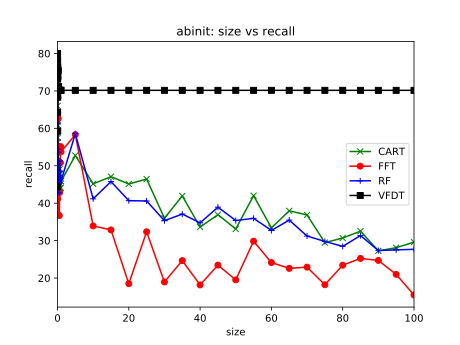
\includegraphics[width=6cm,height=4cm,keepaspectratio]{fig/abinit-size-recall.png}
	\caption{Size vs Recall for abinit dataset}
	\label{fig:ab-size-rec}
\end{figure}

From the figure \ref{fig:ab-size-prec} and \ref{fig:ab-size-prec} it can be seen that, with increase of the examples in abinit dataset, precision score for VFDT does not fluctuate but for the other three learners, it fluctuates, mostly FFT. However, in case of recall score, VFDT performs far better and stable across all of the sizes for the dataset. For the other three learners, the score gets lower and lower when the size increases. 

\begin{figure}[h]
	\includegraphics[width=6cm,height=4cm,keepaspectratio]{fig/lammps-size-precision.png}
	\caption{Size vs Precision for lammps dataset}
	\label{fig:lm-size-prec}
\end{figure}

\begin{figure}[h]
	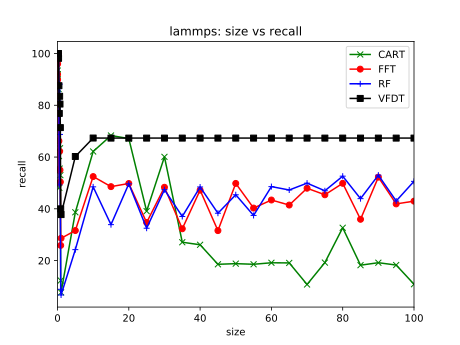
\includegraphics[width=6cm,height=4cm,keepaspectratio]{fig/lammps-size-recall.png}
	\caption{Size vs Recall for lammps dataset}
	\label{fig:lm-size-rec}
\end{figure}

From the figure \ref{fig:lm-size-prec} and \ref{fig:lm-size-prec} it can be seen that, with increase of the examples in lammps dataset, precision score for all the learners are similar and CART is performing slightly better than the others However, in case of recall score, VFDT slightly performs far better and stable across all of the sizes for the dataset. For the other three learners, the score fluctuates back and forth. However, CART performs the worst among the four learners. 

\begin{figure}[h]
	\includegraphics[width=6cm,height=4cm,keepaspectratio]{fig/libmesh-size-precision.png}
	\caption{Size vs Precision for libmesh dataset}
	\label{fig:lb-size-prec}
\end{figure}

\begin{figure}[h]
	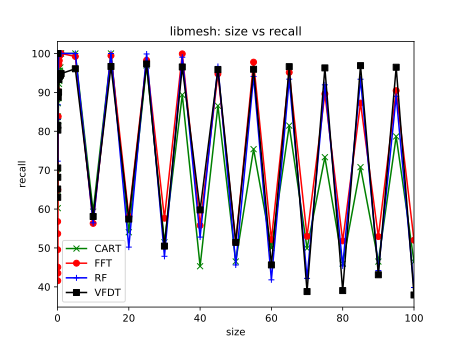
\includegraphics[width=6cm,height=4cm,keepaspectratio]{fig/libmesh-size-recall.png}
	\caption{Size vs Recall for libmesh dataset}
	\label{fig:lb-size-rec}
\end{figure}

From the figure \ref{fig:lb-size-prec} and \ref{fig:lb-size-prec} it can be seen that, with increase of the examples in libmesh dataset, precision and recall score for all the learners are similar. However, it also shows that with the increase of dataset size, the recall scores behaves very unstable, for all of the four learners. 

\begin{figure}[h]
	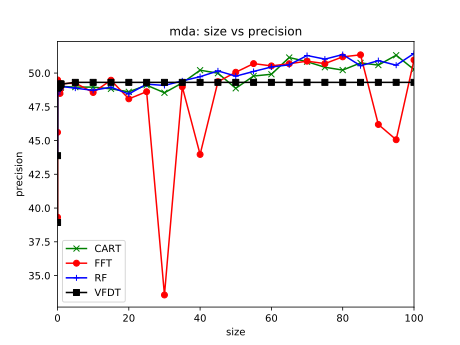
\includegraphics[width=6cm,height=4cm,keepaspectratio]{fig/mda-size-precision.png}
	\caption{Size vs Precision for mdanalysis dataset}
	\label{fig:md-size-prec}
\end{figure}

\begin{figure}[h]
	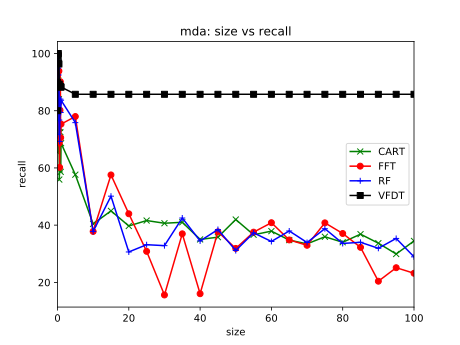
\includegraphics[width=6cm,height=4cm,keepaspectratio]{fig/mda-size-recall.png}
	\caption{Size vs Recall for mdanalysis dataset}
	\label{fig:md-size-rec}
\end{figure}

From the figure \ref{fig:md-size-prec} and \ref{fig:md-size-prec} it can be seen that, with increase of the examples in mdanalysis dataset, precision score for all the learners are similar and CART as well as FFT are performing slightly better than the others However, in case of recall score, VFDT performs far better and stable across all of the sizes for the dataset. For the other three learners, the score fluctuates back and forth a ittle bit. However, FFT performs the worst among the four learners. 

\begin{figure}[h]
	\includegraphics[width=\linewidth]{fig/auc-size.png}
	\caption{AUC of size-recall for all datasets}
	\label{fig:auc-size}
\end{figure}

\begin{figure}
	\centering
	\begin{subfigure}[b]{\linewidth}
		\includegraphics[width=.49\linewidth]{fig/abinit-size-fa.png} \ 
		\includegraphics[width=.49\linewidth]{fig/lammps-size-fa.png}
	\end{subfigure}
	\begin{subfigure}[b]{\linewidth}
		\includegraphics[width=.49\linewidth]{fig/libmesh-size-fa.png} \ 
		\includegraphics[width=.49\linewidth]{fig/mda-size-fa.png}
	\end{subfigure}
	
	\caption{Data Size vs False Alarm}\label{fig:fa}
\end{figure}

From the figure \ref{fig:fa}, it can be seen that false alarm count for all the datasets are higher. It can also be seen that false alarm score is similar to recall score across all the datasets. Hence, confusion matrix of the learners were looked into and it was observed that across all size, the number of True Negatives (TN) and False Negatives (FN) are higher than that of True Positives (TP) and False Positives (FP). Moreover, TN and FN are similar. Theoretically, if the precision score is around $50\%$, then recall score and false alarm score would become similar. This happens because, if precision is around $0.5$, then TP will be similar to FP. So, that will mean, the value of $\frac{TP}{TP+FN}$ and $\frac{FP}{FP+FN}$ will be similar. Thus it can be concluded that, for this particular scope recall and false alarm will be similar. 

In principle, the key observation from the analysis of four datasets are given below: 
\begin{itemize}
	\item VFDT performs better in recall score across all the dataset size. This can also be seen in the AUC score given in \ref{fig:auc-size}
	\item VFDT achieves slightly a lower precision score than the other three learners. This can also be seen in the AUC score given in \ref{fig:auc-size}
	\item Precision and recall scores of all the three learners except VFDT either goes up or down with the increase of data fed into them. For VFDT, it remains stable. As, VFDT reaches hoeffding bound and grows tree accordingly, with the increase of the data size, its tree structure does not change. Hence, its precision and recall score also stay unchanged.
	\item As tuning of the learners was performed with $25\%$ of the examples, it is obvious that optimal parameters for VFDT did not change while newer examples came. But with the arrival of newer examples, optimal set of parameters of CART and RF have changes. This is why their precision and recall score dropped.  
	\item the precision score also tells that all the learner performed marginally better than a random guess. 
	\item High rate of false alarm is a genuine concern. It is also associated with the fact of precision score not getting better than the random guess.
\end{itemize}

\subsection{How hyper-parameter tuning changes the performance as the data size changes}
From the analysis in previous section, it is obvious that when the learner faces substantial amount of newer examples, their prediction performance goes down. Consequently, it remains to be seen whether further parameter tuning improves their performance or not. Moreover, it was understood that, if the false alarm rate needs to decreased, increase in the precision score is needed. So at first parameter tuning was applied to increase the f1 score with very high iteration count. As it is time consuming, parameter tuning was only applied for CART on $25\%$ of the datasets. Initially RF, FFT or VFDT were not chosen because applying parameter tuning on them is time consuming due to the facts mentioned below:

\begin{enumerate}
	\item Tuning was already applied to all the learners on all the datasets across $40$ split size with $10$ random sample of it. Still, decent f1 score was not found. So, there might be a possibility that, any better precision and recall at the same time could not be found. 
	\item FFT is inherently time consuming for discretization on more than $25$ attributes. It is also built from scratched and not as optimized as scikit-learn CART
	\item RF needs to build at least $10$ estimators and thus at least $10$ times expensive than CART
	\item VFDT can be much faster than CART. However, parameter tuning with $n_min$ and $\tau$ can be time consuming as well.
\end{enumerate} 

After running the differential evolution algorithm, it was found out that the best precision score obtained is $0.56$ from \textit{lammps} dataset and worst obtained is $0.48$ from \textit{abinit} dataset. After that, the DE was run once again but with a goal to maximize the difference between recall and false alarm rate. But a maximum difference of $0.07$ in \textit{lammps} dataset was found.

Keeping this in mind, another three parameter tuning was performed while the datasets finished processing $50\%$, $75\%$ and $100\%$ of the total examples. It was observed that precision score does not vary significantly across the dataset size from all the learners, hence in the differential evolution method, it was tried to optimize the parameters on the basis of recall score. Here is the summary of the findings:

\begin{figure}[h]
	\includegraphics[width=\linewidth]{fig/tune-ab.png}
	\caption{Size vs Recall for mdanalysis dataset}
	\label{fig:tune-ab}
\end{figure}

\begin{figure}[h]
	\includegraphics[width=\linewidth]{fig/tune-lm.png}
	\caption{Size vs Recall for mdanalysis dataset}
	\label{fig:tune-lm}
\end{figure}

\begin{figure}[h]
	\includegraphics[width=\linewidth]{fig/tune-lb.png}
	\caption{Size vs Recall for mdanalysis dataset}
	\label{fig:tune-lb}
\end{figure}

\begin{figure}[h]
	\includegraphics[width=\linewidth]{fig/tune-md.png}
	\caption{Size vs Recall for mdanalysis dataset}
	\label{fig:tune-md}
\end{figure}

It is obvious from Figure \ref{fig:tune-ab}, \ref{fig:tune-lm}, \ref{fig:tune-lb}, \ref{fig:tune-md} that, for most of the cases recall score could have been improved if further tuning was deployed after seeing a substantial amount of newer examples. It is also obvious that recall score of VFDT can be improved farther. However, in case of learning for a large stream of data periodically, it is really inefficient to apply tuning each time the dataset learns. 

\subsection{RQ3: How much computation resources would be used by these four learners}
It is also important to observe the computational resources being used by the learners because, with the increase of data size, the need for the learners to become cheap in terms of time and memory is paramount. Here, the findings from the analysis is presented below.

\begin{figure}
	\centering
	\begin{subfigure}[b]{\linewidth}
		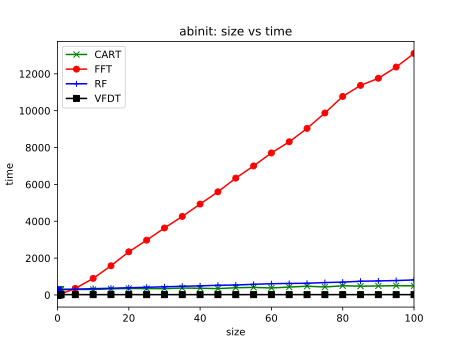
\includegraphics[width=.49\linewidth]{fig/abinit-size-time.png} \ 
		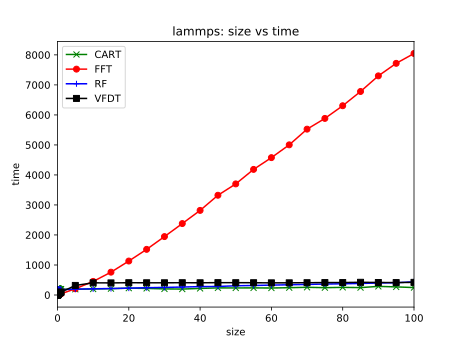
\includegraphics[width=.49\linewidth]{fig/lammps-size-time.png}
	\end{subfigure}
	\begin{subfigure}[b]{\linewidth}
		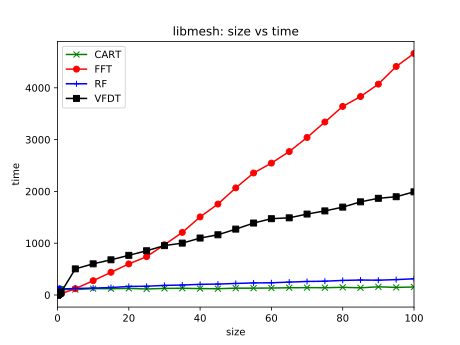
\includegraphics[width=.49\linewidth]{fig/libmesh-size-time.png} \ 
		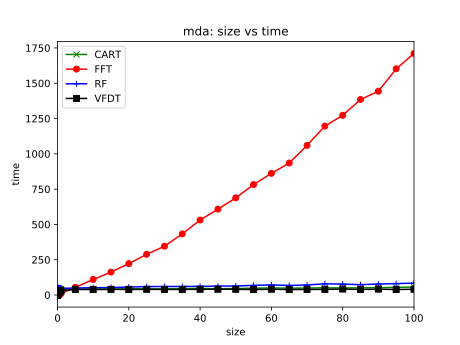
\includegraphics[width=.49\linewidth]{fig/mda-size-time.png}
	\end{subfigure}
	
	\caption{Data Size vs Time}\label{fig:time}
\end{figure}

From the above fig \ref{fig:time}, it can be seen that FFT is very expensive in terms of computation time. Apart from libmesh dataset, it is also seen that CART, RF and VFDT all takes similar time to operate. However, such comparison between VFDT, CART and RF is not conclusive as the dataset is very small compared to the available primary memory in the testbed system. Hence, it was needed to deploy the learner with a very big dataset that is similar to the size of primary memory of the computer. Unfortunately, such big dataset is not available for software defect prediction. Hence, a huge physics dataset for atomic particles was collected from UCI Machine Learning dataset repository \cite{uciml}. The size of the dataset is around $8$Gb of size. It contains $110000000$ rows and $29$ columns. All the class labels are either boolean and attributes are continuous. From the run, here is the outcome. From the table \ref{higgs} above, it is obvious that VFDT scales in terms of both computation time and memory usage if the dataset size is substantially large.

\begin{table}
	\begin{tabular}{|c|c|c|}
		\hline 
		\textbf{Learner} & \textbf{Time} & \textbf{Memory} \\ 
		\hline 
		CART & 332 sec & 6.1 GB \\ 
		\hline 
		RF & 425 sec & 6.1 GB \\ 
		\hline 
		VFDT & 34 sec & 271 MB \\ 
		\hline 
	\end{tabular}
	\caption{Computation Resource Usage for Very Large Dataset} 
	\label{higgs}
\end{table}

\subsection{Revisiting Baseline Criteria: }
The initital motivation is to observe whether stream based VFDT can do better than the offline classifiers. Hence, based on the observation above, here is the observation from the aspect of the aforementioned baseline.
\begin{enumerate}
	\item \textbf{Useful: } In terms of precision, no learner is useful as those are not better than random guess significantly. However, in terms of recall, VFDT have outperformed others.
	\item \textbf{Reasonable: } VFDT has performed no worse than the other established learners in this case.
	\item \textbf{Stable: } VFDT has shown much more stable result than the other three
	\item \textbf{Robust: } Across different datasets and splits, VFDT has shown more robust performance than the other three.
	\item \textbf{Cheap: } VFDT is computationally cheaper than the others.
	\item \textbf{Streaming: } VFDT can handle large datasets sequentially and it does not need to load the whole set of examples to primary memory.
	\item \textbf{Tunable: } Parameter tuning yielded better recall rates for VFDT than the others across all the sizes.
\end{enumerate}

\section{Threats to Validity}
\begin{enumerate}
	\item \textbf{Sampling Bias: } Like every classification experiment, this work is also subject to have some bias in sampling training and test data. Although $10$ disjoint training and testing datasets for each dataset was sampled, it could have been better if the sampling number was higher
	\item \textbf{Random Bias: } Some of the learners in the experiments utilized random value generation such as RF. Rerunning such classifiers multiple times could given a less biased outputs.
	\item \textbf{Parameter Bias: } In differential evolution algorithm, some parameters were used to find the best parameters for the learners. So inherently, the tuning method also suffers from some degree of biasness induced by the parameters in the tuning algorithms.
	\item \textbf{Code Optimization: } Program written from scratch for VFDT and FFT are not as optimized as the CART and RF from scikit-learn package. So the experiment for computational resource could have been bias free if RF and CART were built from the scratch as well.
	\item \textbf{Dataset: } The experiment performed is only based on the four datasets. It should also be conducted on other large defect datasets to get a more neutral perception.
	\item \textbf{Cross Validation: } The performance of the learners could have been better observed if cross-validation was performed. However, as the data is ordered, it was not possible.
\end{enumerate}

\section{Future Work Direction and Conclusion}
Despite the fact that, VFDT has gained in all the baseline criteria that are looked into so far, it has also opened several future work directions. Firstly, the experiment should also be performed in other large software defect datasets to gain even better understanding. Second, the issue of high rate of false alarm should be probed. Moreover, using multi-threading and multi-processing, VFDT can be made much more faster as well. Finally, C-VFDT \cite{hulten2001mining} - which is a variant of VFDT can be much more useful in the defect prediction scenario as it can change its tree structure due to any potential distribution change or concept drift in large dataset \cite{vzliobaite2010learning} - can be deployed in defect prediction and the performance should be observed.

%% Bibliography
\bibliography{bibfile}
\bibliographystyle{ACM-Reference-Format}
%
%
%%% Appendix
%\appendix
%\section{Appendix}


\end{document}
